%%%%%%%%%%%%%%%%%%%%%%%%%%%%%%%%%%%%%%%%%%%%%%%%%%%%%%%%%%%%
\subsubsection*{Neutrinoless double beta decay and Majorana neutrinos}

Neutrinos, unlike the other Standard Model fermions, could be Majorana particles, that is, indistinguishable from their antiparticles. The existence of Majorana neutrinos would have profound implications in particle physics and cosmology. If neutrinos are Majorana particles, there must exist a new scale of physics the level of which is inversely proportional to neutrino masses, that characterises new underlying dynamics beyond the Standard Model. The existence of such a new scale provides the simplest explanation of why neutrino masses are so much lighter than the charged fermions. Understanding the new physics that underlies neutrino masses is one of the most important open questions in particle physics. It could have profound implications in our understanding of the mechanism of symmetry breaking, the origin of mass and the flavour problem.

Furthermore, the existence of Majorana neutrinos would imply that lepton number is not a conserved quantum number which could be the origin of the matter-antimatter asymmetry observed in the Universe. The new physics related to neutrino masses could provide a new mechanism to generate the asymmetry, called leptogenesis. 

The only practical way to establish experimentally that neutrinos are their own antiparticle is the detection of neutrinoless double beta decay (\bbonu). This is a postulated very slow radioactive process in which a nucleus with $Z$ protons decays into a nucleus with $Z+2$ protons and the same mass number $A$, emitting two electrons that carry essentially all the energy released (\Qbb). The process can occur if and only if neutrinos are massive, Majorana particles.

Several underlying mechanisms --- involving, in general, physics beyond the Standard Model  --- have been proposed for \bbonu, the simplest one being the virtual exchange of light Majorana neutrinos. Assuming this to be the dominant process at low energies, the half-life of \bbonu\ can be written as
\begin{equation}
(T^{0\nu}_{1/2})^{-1} = G^{0\nu} \ \big|M^{0\nu}\big|^{2} \ \mbb^{2} \, .
\label{eq:Tonu}
\end{equation}
In this equation, $G^{0\nu}$ is an exactly-calculable phase-space integral for the emission of two electrons; $M^{0\nu}$ is the nuclear matrix element (NME) of the transition, which has to be evaluated theoretically; and \mbb\ is the \emph{effective Majorana mass} of the electron neutrino:
\begin{equation}
\mbb = \Big| \sum_{i} U^{2}_{ei} \ m_{i} \Big| \, ,
\end{equation}
where $m_{i}$ are the neutrino mass eigenstates and $U_{ei}$ are elements of the neutrino mixing matrix. Therefore, a measurement of the decay rate of \bbonu\ would provide direct information on neutrino masses.

The relationship between \mbb\ and the actual neutrino masses $m_i$ is affected by the uncertainties in the measured oscillation parameters, the unknown neutrino mass ordering (normal or inverted), and the unknown phases in the neutrino mixing matrix (both Dirac and Majorana). The current knowledge on neutrino masses and mixings provided by neutrino oscillation experiments is summarized in the left panel of fig.~\ref{fig:numass_ordering}. The diagram shows the two possible mass orderings that are compatible with neutrino oscillation data, with increasing neutrino masses from bottom to top. The relationship between \mbb\ and the lightest neutrino mass $m_{\rm light}$ (which is equal to $m_1$ or $m_3$ in the normal and inverted mass orderings, respectively) is illustrated in the right panel of Fig.~\ref{fig:numass_ordering}.

%%%%%%%%%%
\begin{figure}[h]
\centering
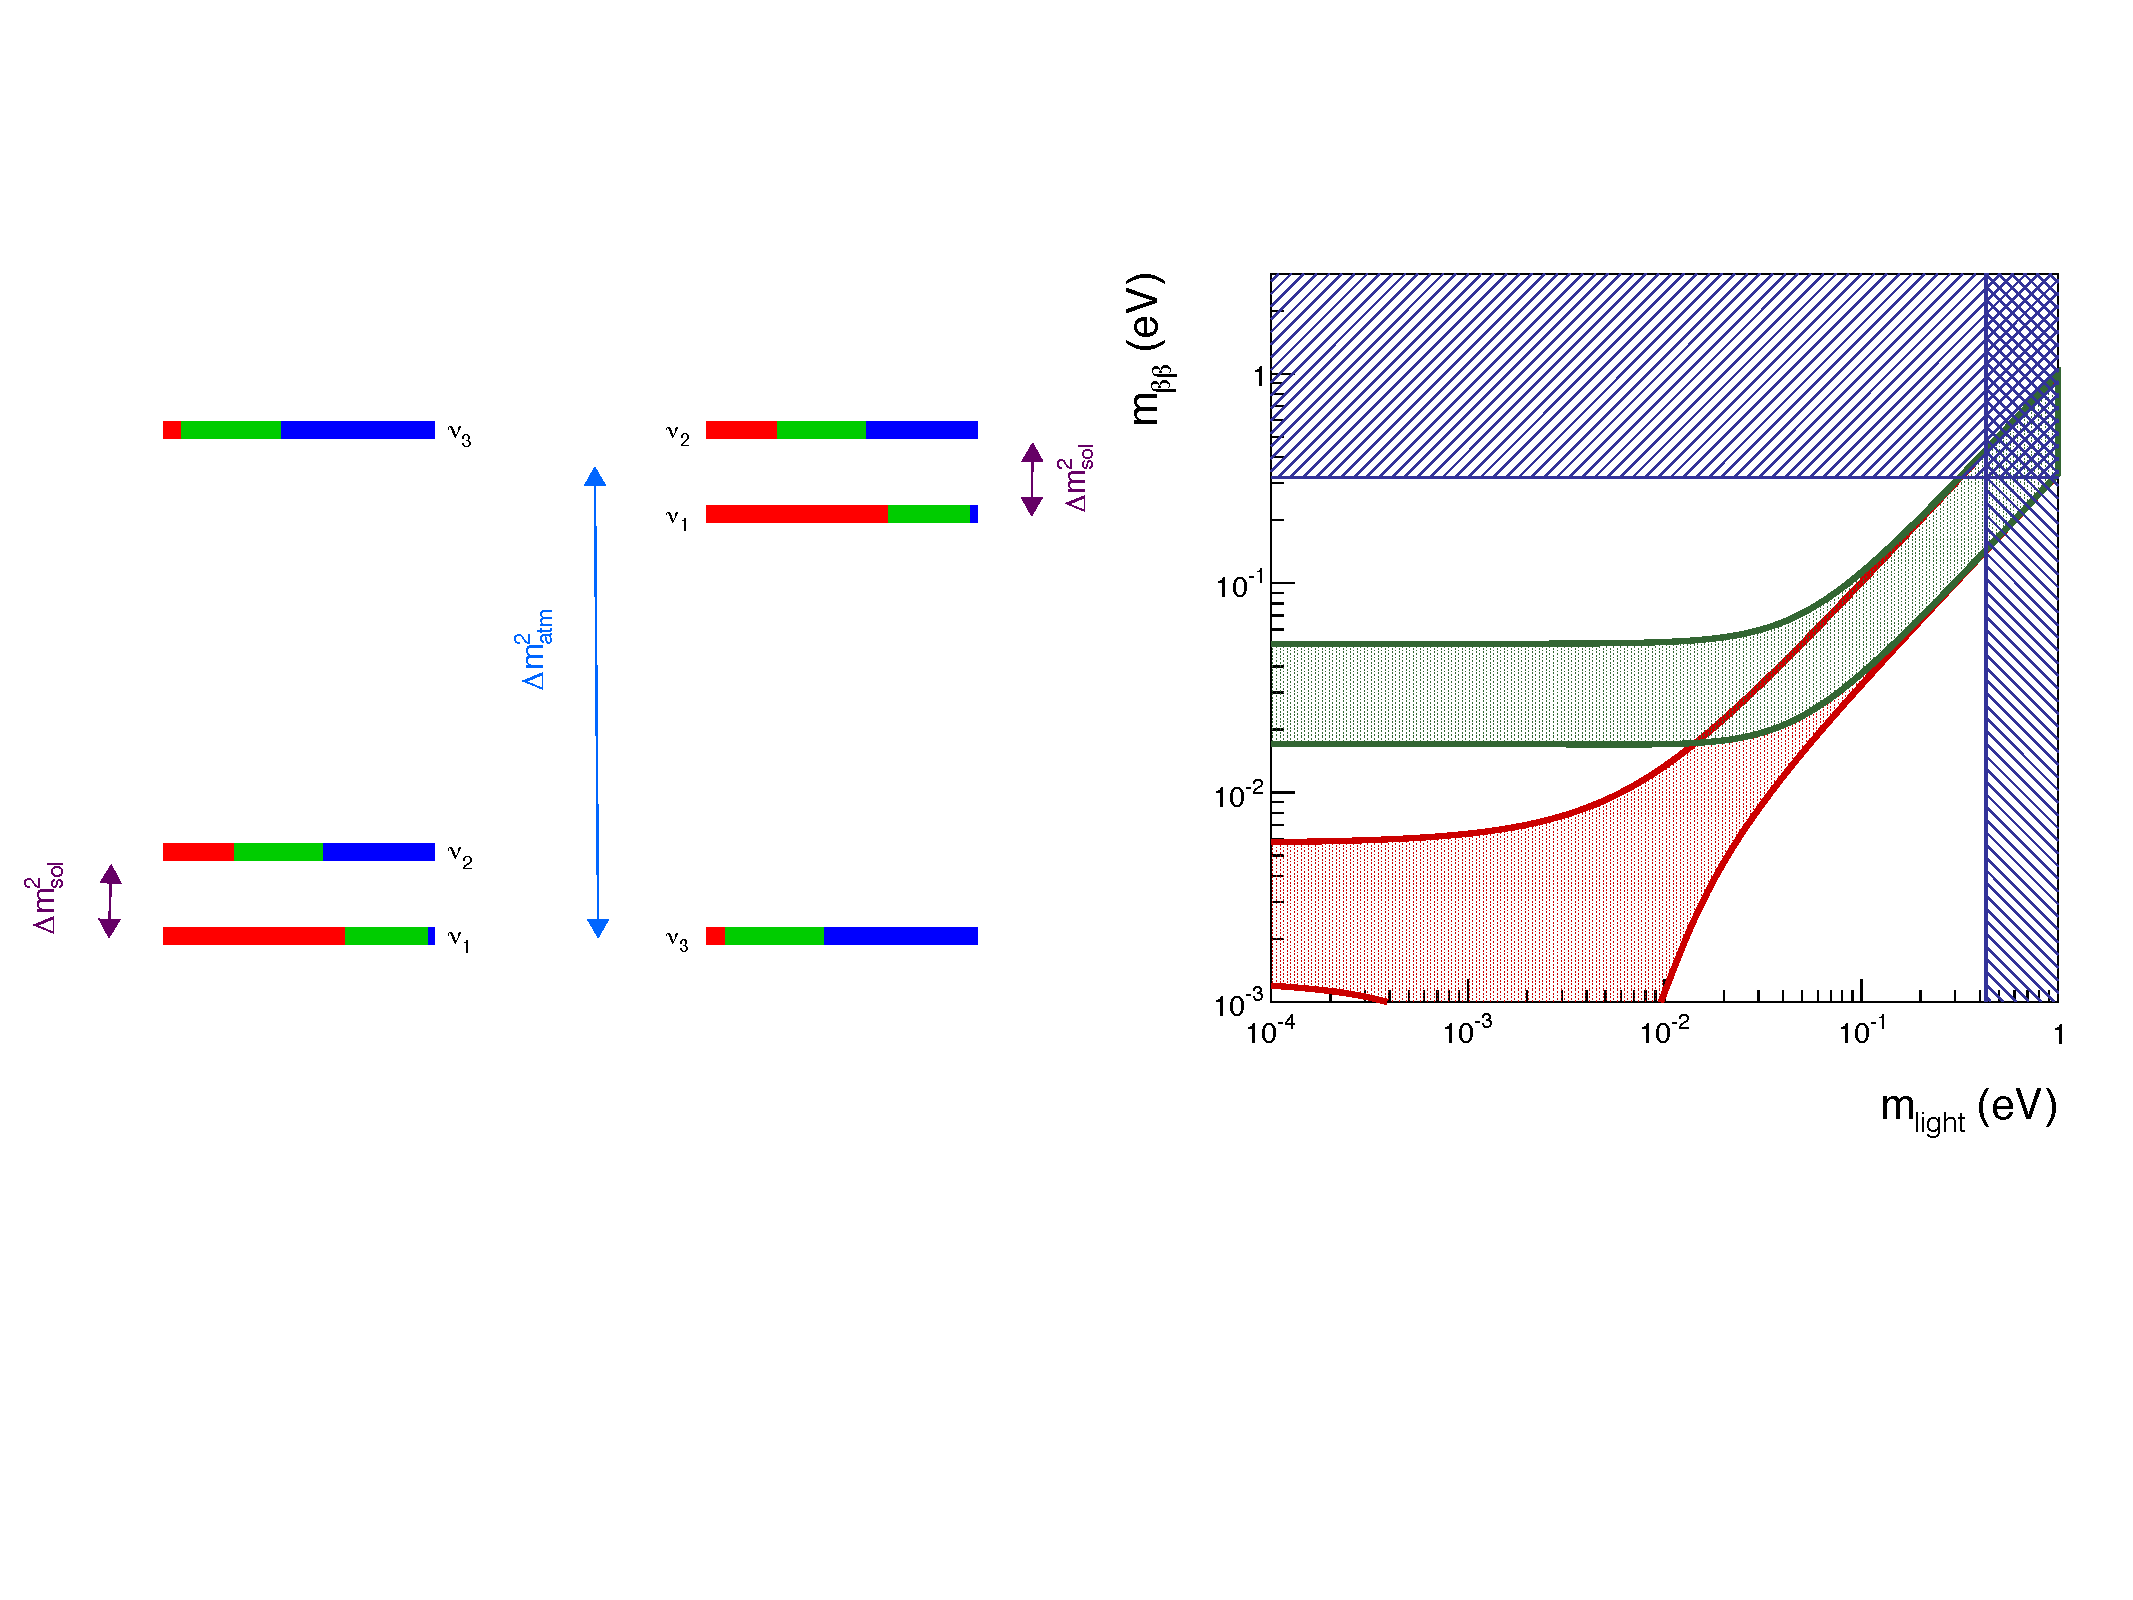
\includegraphics[width=0.99\textwidth]{img/numassmix.pdf}
\caption{\small The left panel shows the normal (left) and inverted (right) mass orderings. The electron, muon and tau flavor content of each neutrino mass eigenstate is shown via the red, green and blue fractions, respectively. The right panel shows the effective neutrino Majorana mass, \mbb, as a function of the lightest neutrino mass, $m_{\rm light}$. The green band corresponds to the inverse hierarchy of neutrino masses, whereas the red corresponds to the normal ordering. The upper bound on the lightest neutrino mass comes from cosmological bounds; the bound on the effective Majorana mass from \bbonu\ constraints.} \label{fig:numass_ordering}
\end{figure}
%%%%%%%%%%

The upper bound on the effective Majorana mass corresponds to the experimental constraint set by the Heidelberg-Moscow (HM) experiment, which was until very recently the most sensitive limit to the half-life of \bbonu: $T^{0\nu}_{1/2}(\GE) \ge 1.9\times10^{25}$ years at 90\% CL.\footcite{KlapdorKleingrothaus:2000sn}  A subgroup of the HM experiment interpreted the data as {\em evidence} of a positive signal, with a best value for the half-life of $1.5\times10^{25}$ years, corresponding to an effective Majorana mass of about 400 meV.\footcite{KlapdorKleingrothaus:2001ke} This claim  was very controversial and still awaits a definitive experimental response.


%%%%%%%%%%%%%%%%%%%%%%%%%%%%%%%%%%%%%%%%%%%%%%%%%%%%%%%%%%
\subsubsection*{Experimental aspects}

The detectors used in double beta decay searches are designed, primarily, to measure the energy of the radiation emitted by a \bb\ source to high precision. In the case of \bbonu, the sum of the kinetic energies of the two released electrons is always the same, and is equal to the mass difference between the parent and the daughter nuclei: $Q_{\bb} \equiv M(Z,A)-M(Z+2,A)$. However, due to the finite energy resolution of any detector, \bbonu\ events are reconstructed within a non-zero energy range centered around \Qbb, typically following a Gaussian distribution. Important backgrounds are those events in the detector of origin not related to \bbonu\ which are reconstructed with energies within this range.

All double beta decay experiments have to deal with an intrinsic background, the standard \bbtnu\ (a SM-allowed process consisting in two simultaneous $\beta$ decays), that can only be suppressed by achieving an energy resolution sufficiently good to separate the continuous spectrum of \bbtnu\ from the Gaussian \bbonu. Backgrounds of cosmogenic origin force the underground operation of the detectors. However, natural radioactivity emanating from the detector materials and surroundings still have the potential to overwhelm the signal peak and hence careful selection of radiopure materials is essential. Additional experimental signatures that allow the distinction of signal and background can further strengthen a result.

Besides energy resolution and control of backgrounds, several other factors such as detection efficiency and the scalability to large masses must be taken into account in the design of a double beta decay experiment. The simultaneous optimization of all these parameters is often challenging, if not impossible, and consequently many different experimental approaches have been proposed. In order to compare them the experimental sensitivity to \mbb is used as a figure of merit:\footcite{GomezCadenas:2010gs}
%%%
\begin{equation}
\mbb = K \ \sqrt{1/\varepsilon} \ \left(\frac{b\cdot\Delta E}{M\cdot t} \right)^{1/4}\, ,
\label{eq:mbb}
\end{equation}
%%%
where $\varepsilon$ is the detection efficiency, $\Delta E$ is the energy resolution window where the \bbonu\ signal will be reconstructed, $b$ is the background rate (in counts per year, kilogram of \bb\ isotope, keV) in the region of interest, $M$ is the \bb\ isotope mass, and $t$ is the data-taking time. 


%%%%%%%%%%%%%%%%%%%%%%%%%%%%%%%%%%%%%%%%%%%%%%%%%%%%%%%%%%
\subsubsection*{The current generation of xenon-based \bbonu\ experiments}
 
 Two xenon-based experiments are currently leading the field: KamLAND-Zen, in which xenon is dissolved in liquid scintillator and EXO-200, a liquid xenon (LXe) TPC. Both have recently published negative results. 
 EXO achieves an energy resolution of 4\% FWHM at \Qbb, and a background rate measured in the \emph{region of interest} (ROI) of $ 4 \times 10^{-3}\ckky$. The total exposure used for the published result is 100 kg$\cdot$year. They have published a limit on the half-life of \bbonu\ of $T_{1/2}^{0\nu}(\XE) > 2 \times 10^{25}$ years.\footcite{Auger:2012ar} 
KamLAND-Zen compensates a worse energy resolution of 10\% FWHM at \Qbb\ with an exposure three times larger, 89.5 kg year. They have published a limit on the half-life of \bbonu\ of $T_{1/2}^{0\nu}(\XE) > 1.9 \times 10^{25}$ years.\footcite{Gando:2012zm} In terms of the effective neutrino mass, the EXO Collaboration quotes a sensitivity ranging between 140 and 380 meV, and KamLAND-Zen quotes a sensitivity ranging between 120 and 250 meV. 


%%%%%%%%%%%%%%%%%%%%%%%%%%%%%%%%%%%%%%%%%%%%%%%%%%%%%%%%%%
